\documentclass[captions=tableheading]{scrartcl}

\usepackage{amsmath}
\usepackage{amssymb}
\usepackage[utf8]{inputenc}
\usepackage[T1]{fontenc}
\usepackage{lmodern}
\usepackage{ngerman}
\usepackage{geometry}
\usepackage{graphicx}
\usepackage{wrapfig}
\usepackage{caption}
\usepackage{wasysym}
\usepackage[separate-uncertainty=true]{siunitx}
\usepackage{picinpar}
\usepackage{tikz}
\usepackage{float}
\usepackage{booktabs}
\usepackage{enumitem} 

\renewcommand{\figurename}{Abb.}
\usepackage[
	colorlinks=true,
	urlcolor=blue,
	linkcolor=black
]{hyperref}


%Hier Titel und so
\newcommand{\versuchnummer}{} 
\newcommand{\versuchname}{Röntgenreflektometrie} 
\newcommand{\versuchdatum}{16.02.2017} 
\newcommand{\im}{\mathrm{i}}
\newcommand{\indx}[1]{\text{#1}}
\newcommand{\RE}[1]{\mathrm{Re} \left(#1 \right)}


\title{Versuch \versuchnummer\\ \versuchname}
\subtitle{Physikalisches Fortgeschrittenenpraktikum}
\author{Robert Rauter und Björn Lindhauer}
\date{\versuchdatum} 
\begin{document}
\begin{titlepage}
{\large \versuchdatum}
\vspace{7cm}
\begin{center}
\textbf{\huge Versuch \versuchnummer}\\\vspace{0.5cm}
\textbf{\huge \versuchname}\\
\vspace{0.2cm}
\textbf{Physikalisches Fortgeschrittenenpraktikum}\\
\vspace{9cm}

{\Large Robert Rauter \ \ \hspace{1.5cm} und \hspace{1.5cm} Björn Lindhauer}\\
{ \url{robert.rauter@tu-dortmund.de} \ \ \hspace{2cm} \url{bjoern.lindhauer@tu-dortmund.de}}
\end{center}
\end{titlepage}

\section{Theoretische Grundlagen}
Bei der Röntgenreflektometrie werden elektromagnetische Welle mit Wellenlänge $\lambda=$ \SIrange{0.1}{10}{\angstrom} und Feldvektor 
\begin{equation}
E\left(r\right)=E_0 \exp\left(\im  k\cdot r \right)
\end{equation}
betrachtet, die aus dem Vakuum mit Brechungsindex $n_1=1$ auf ein Medium mit Brechungsindex $n_2:=n \neq 1$ trifft.

Bei Röntgenstrahlen ist der Realteil des Brechungsindex $n$ geringfügig kleiner als 1, da die Schwingungsfrequenz von Röntgenstrahlung höher ist als die Resonanzfrequenz von Elektronen in einem Medium.
Ist der Realteil des Brechungsindexes kleiner eins, so ist die Phasengeschwindigkeit größer als die Lichtgeschwindigkeit $c$.
Dies ist kein Widerspruch zur Relativitätstheorie, da die relavante Geschwindigkeit für Informationsaustausch die Gruppengeschwindigkeit ist und diese natürlich unter der Lichtgeschwindigkeit liegt.

Weil der Brechungsindex nahe Eins liegt, wird er häufig als
\begin{equation}
n=1-\delta + \im\beta \hspace{0.5cm}\text{,}\hspace{0.1cm} \delta >0
\end{equation}
geschrieben. 
Die Korrektur $\delta$ liegt in der Größenordnung $10^{-6}$. 
Die Absorption wird durch den Parameter $\beta$ beschrieben und liegt für Röntgenstrahlen der Energie $E=$\SI{8}{\kilo\eV} bei $\beta \sim 10^{-7}$.

\subsection{Einschichtsystem}
In diesen Abschnitt wird zunächst die Reflexion der Röntgenstrahlen an einer homogenen Schicht betrachtet.
Die elektromagnetische Welle trifft auf die Oberfläche der homogenen Schicht und wird wie in Abbildung \ref{fig:reflexionschicht} dargestellt, teilweise reflektiert und teilweise gebrochen.
\begin{center}
	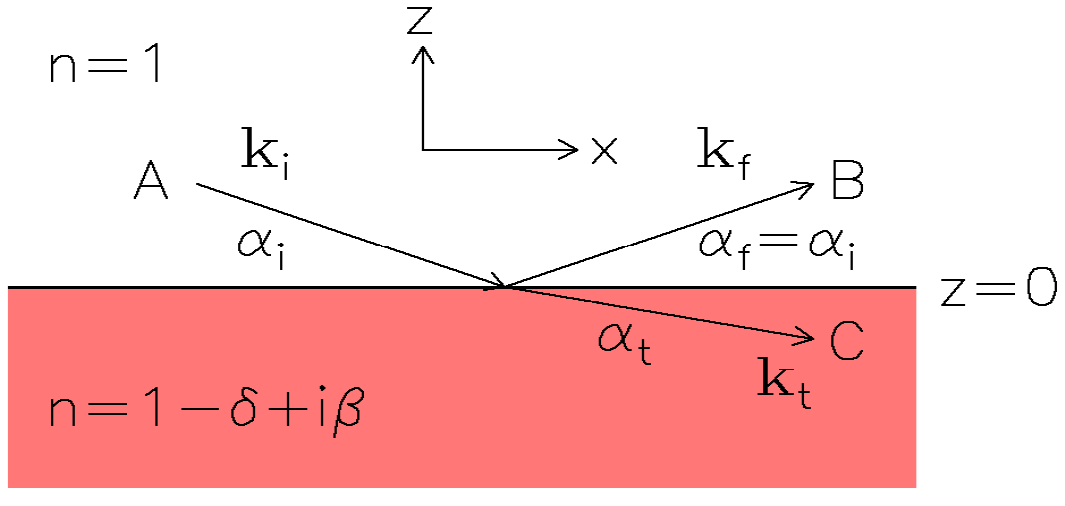
\includegraphics[width=10cm]{images/reflexionschicht.png}
	\captionof{figure}{Graphische Darstellung der einfallenden, teflexierten und gebrochenen Strahlen an einer Grenzschicht mit unterschiedlichen Brechungsindex. \ref{q:anleitung}}
	\label{fig:reflexionschicht}
\end{center}
Es kann in diesen Fall das Brechungsgesetz nach Snellius angewendet werden, nur ist zu beachten, dass die Winkel aufgrund ihrer kleinen Größe im Bezug zur Oberfläche und nicht im Bezug auf das Lot gemessen werden. 
Dies führt zu einer Phasenverschiebung von $\frac{\pi}{2}$ in den trigonometrischen Funktionen.
Somit lautet das Brechungsgesetz nach Snellius
\begin{equation}
\cos \alpha_{\indx{i}}=n\cos \alpha_{\indx{t}} \hspace{0.5cm}\text{.}
\end{equation}
Dies hat zur Folge, dass es aufgrund von $\RE{n}<1 $ ein kritischer Winkel
\begin{equation}
\alpha_{\indx{c}}=\arccos n \approx \sqrt{2\delta } = \lambda \sqrt{\frac{r_{\indx{e}} \rho}{\pi}}
\end{equation}
existiert, ab dem $\alpha \le \alpha_{\indx{c}}$ nur noch Totalreflexion auftritt.
Dabei ist $\lambda$ die Wellenlänge der Röntgenstrahlung, $r_{\indx{e}}$ der klassische Elektronenradius und $\rho$ die Elektronendichte des Materials. 

Wie in der Optik gelten die Fresnelformeln für s-polarisierte Strahlung
\begin{equation}
r_{\indx{s}}= \frac{B}{A}= \frac{k_{\indx{i}}^{\left(z\right)}-k_{\indx{t}}^{\left(z\right)}}{k_{\indx{i}}^{\left(z\right)}+k_{\indx{t}}^{\left(z\right)}}
\end{equation}
\begin{equation}
t_{\indx{s}}= \frac{C}{A}= \frac{2k_{\indx{i}}^{\left(z\right)}}{k_{\indx{i}}^{\left(z\right)}+k_{\indx{t}}^{\left(z\right)}}
\end{equation}
und für die p-polarisierte Strahlung 
\begin{equation}
r_{\indx{p}}= \frac{B}{A}= \frac{n^2 k_{\indx{i}}^{\left(z\right)}- k_{\indx{t}}^{\left(z\right)}}{k_{\indx{i}}^{\left(z\right)}+k_{\indx{t}}^{\left(z\right)}}
\end{equation}
\begin{equation}
t_{\indx{p}}= \frac{C}{A}= \frac{2nk_{\indx{i}}^{\left(z\right)}}{n^2k_{\indx{i}}^{\left(z\right)}+k_{\indx{t}}^{\left(z\right)}}
\end{equation}
mit $k_{\indx{i}}^{\left(z\right)}=k\sin \alpha_{\indx{i}}$ der z-Koordinate der einfallenden Welle und $k_{\indx{t}}^{\left(z\right)}=nk\sin \alpha_{\indx{t}}$ der z-Koordinate der transmittierten Welle.

Da für Röntgenstrahlen der Brechungsindex $n\approx 1$ ist, kann ein gemeinsamer Transmissions- und Reflexionskoeffizient 
\begin{equation}
r= \frac{B}{A}= \frac{k_{\indx{i}}^{\left(z\right)}- k_{\indx{t}}^{\left(z\right)}}{k_{\indx{i}}^{\left(z\right)}+k_{\indx{t}}^{\left(z\right)}}
\end{equation}
\begin{equation}
t= \frac{C}{A}= \frac{2k_{\indx{i}}^{\left(z\right)}}{k_{\indx{i}}^{\left(z\right)}+k_{\indx{t}}^{\left(z\right)}}
\end{equation}
für s- und p-polarisierte Strahlung verwendet werden. 

Die messbare Intensität ist durch
\begin{equation}
R_{\indx{F}  }=\frac{I_{\indx{R}}}{I_{\indx{0}}}= \left\vert r \right\vert^2
\end{equation}
gegeben.
Wird der Einfallwinkel der Röntgenstrahlung so gewählt, dass $\alpha_{\indx{i}}>3\alpha_{\indx{c}}$ ist, so ist $R_{\indx{F}  }$ näherungsweise durch
\begin{align}
R_{\indx{F}}&=\left\vert r \right\vert^2=\left( \frac{k\sin \alpha_{\indx{i}}  - k\sqrt{ \cos^2 \alpha_{\indx{c}} - \cos^2 \alpha_{\indx{i}} }}{k\sin \alpha_{\indx{i}}  + k\sqrt{ \cos^2 \alpha_{\indx{c}} - \cos^2 \alpha_{\indx{i}} }}  \right)^2\\
&\approx \left( \frac{\alpha_{\indx{i}}-\sqrt{1-\alpha_{\indx{c}}^2 -1 + \alpha_{\indx{i}}^2} }{\alpha_{\indx{i}}+\sqrt{1-\alpha_{\indx{c}}^2 -1 + \alpha_{\indx{i}}^2}}  \right)^2=\left( \frac{1-\sqrt{ 1 -\left(\frac{\alpha_{\indx{c}} }{\alpha_{\indx{i}}}\right)^2}  }{1+\sqrt{ 1 -\left(\frac{\alpha_{\indx{c}} }{\alpha_{\indx{i}}}\right)^2} }  \right)^2\\
&\approx \left( \frac{1-1+\frac{1}{2}\left(\frac{\alpha_{\indx{c}} }{\alpha_{\indx{i}}}\right)^2 }{1+1-\frac{1}{2}\left(\frac{\alpha_{\indx{c}} }{\alpha_{\indx{i}}}\right)^2}  \right)^2= \left(\frac{\left(\frac{\alpha_{\indx{c}} }{\alpha_{\indx{i}}}\right)^2}{4-\left(\frac{\alpha_{\indx{c}} }{\alpha_{\indx{i}}}\right)^2} \right)^2\approx \left(\frac{1}{4}\left(\frac{\alpha_{\indx{c}} }{\alpha_{\indx{i}}}\right)^2   \right)^2\\
&= \left(\frac{\alpha_{\indx{c}} }{2\alpha_{\indx{i}}}\right)^4
\end{align}
gegeben.
\subsection{Mehrschichtsystem}
Durch Interferenz von Strahlen, die in unterschiedlichen Schichten reflektiert wurden, entstehen bei Mehrschichtsystemen Modulationen, die sogenannten Kiessig-Ringe.
Ist der Gangunterschied ein Vielfaches der halben Wellenlänge, so entsteht ein Interferenzmimimum. 
Bei einer Schichtdicke von $d$ gilt
\begin{equation}
2d\sin \alpha_{\indx{i}} =n\lambda
\end{equation}
\begin{equation}
d=\frac{2\pi}{\Delta q}\approx \frac{\lambda}{2\Delta\alpha_{\indx{i}}}\text{,}
\end{equation}
mit $q=2k\sin \alpha_{\indx{i}}$ der Wellenübertrag in z-Richtung. In Abbildung \ref{fig:reflexionschichten} ist dies illustriert.
\begin{center}
	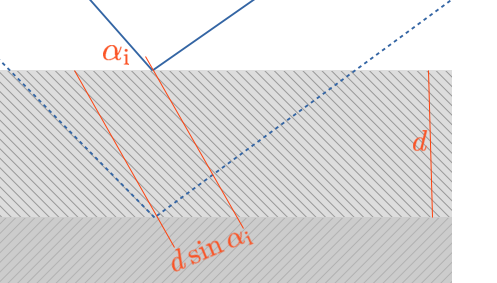
\includegraphics[width=10cm]{images/reflexionschichten.png}
	\captionof{figure}{Schematische Darstellung der destruktiven Interferenz an einem Zweischichtsystem.}
	\label{fig:reflexionschichten}
\end{center}
\begin{center}
	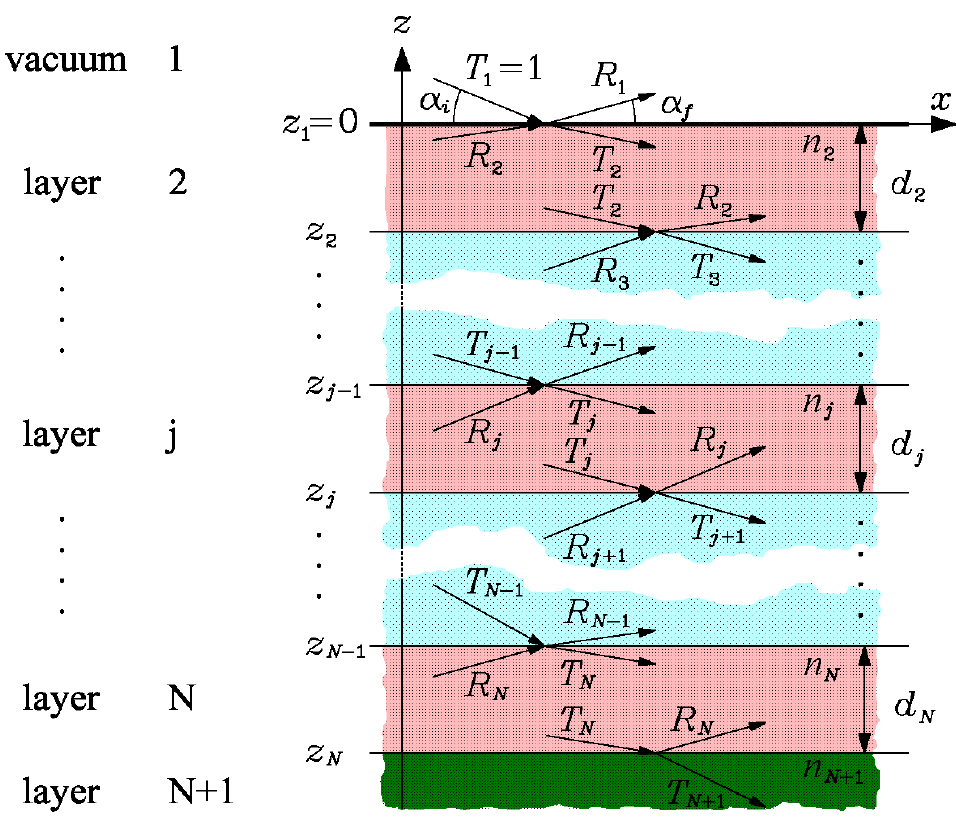
\includegraphics[width=10cm]{images/reflexionmehrschichten.png}
	\captionof{figure}{Schematische Darstellung der Reflexion und Transmission von Röntgenstrahlung
aus dem Vakuum an einem Mehrschichtsystem.  \ref{q:anleitung}}
	\label{fig:reflexionmehrschichten}
\end{center}
Für ein System mit $N$ Schichten, wie in Abbildung \ref{fig:reflexionmehrschichten} kann die Röntgenrefektivität durch den Parratt-Algorithmus berechnet werden. 
Dieser berechnet rekursiv das Verhältnis der reflektierten und transmittierten Wellen an der j-ten Gränzfläche durch
\begin{equation}
X_\indx{j}=\frac{\indx{j}}{T_\indx{j}}=\exp \left(-2\im k_\indx{z,j}z_\indx{j} \right)\frac{r_\indx{j,j+1} + X_\indx{j+1}\exp\left(-2\im k_\indx{z,j+1}z_\indx{j}\right) }{ 1+r_\indx{j,j+1}X_\indx{j+1}\exp\left(-2\im k_\indx{z,j+1}z_\indx{j}\right) }
\end{equation}
mit
\begin{equation}
r_\indx{j,j+1}= \frac{k_\indx{z,j}-k_\indx{z,j+1}}{k_\indx{z,j}+k_\indx{z,j+1}}
\end{equation}
der Fresnelreflektivität der j-ten Grenzfläche. 
Abbildung \ref{fig:reflexionbeispiel} zeigt das Ergebnis des Parratt-Algorithmus für ein System mit einer Schicht mit $\delta=10^{-6}$ auf einen  Substrat mit $\delta = 3\cdot 10^{-6}$.
\begin{center}
	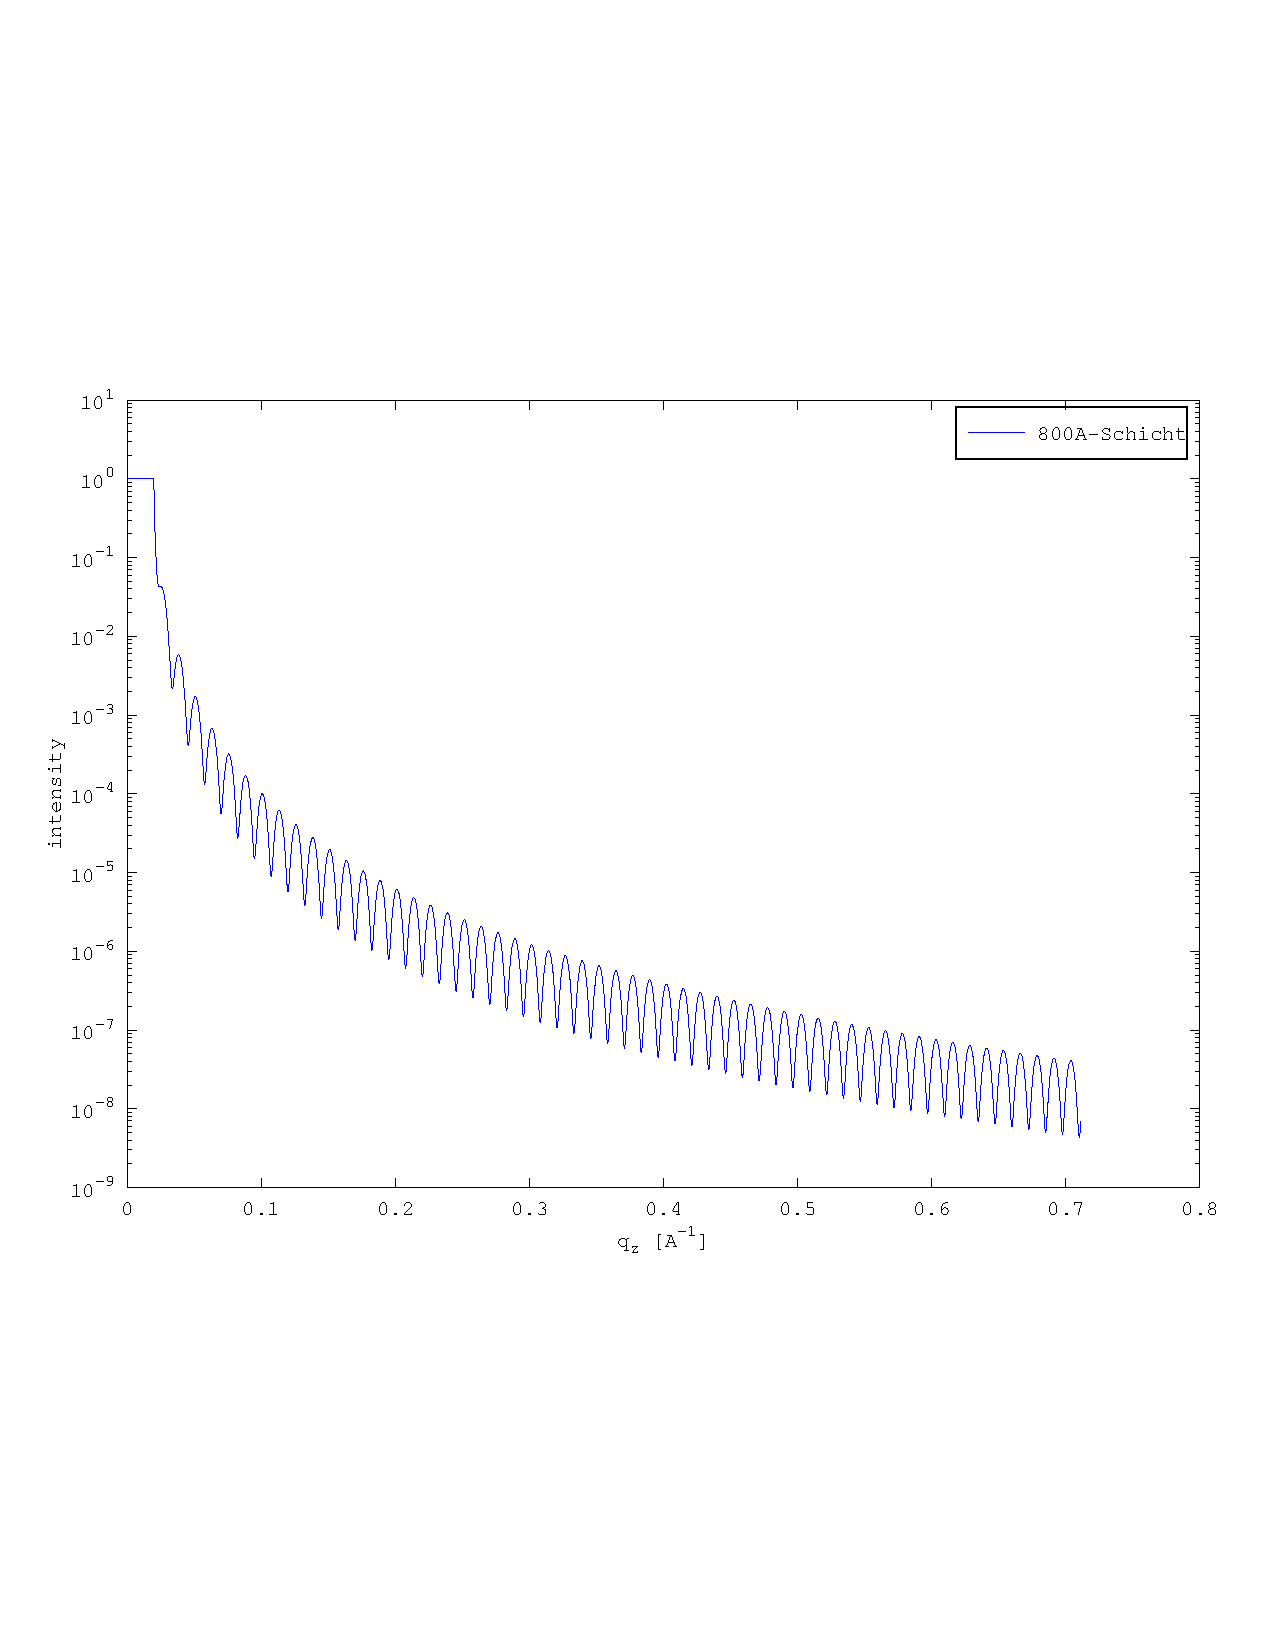
\includegraphics[width=10cm]{images/reflektivitaet_schicht.pdf}
	\captionof{figure}{Durch  Parratt-Algorithmus berechnete Reflexität für ein System mit einer Schicht mit $\delta=10^{-6}$ auf einen  Substrat mit $\delta = 3\cdot 10^{-6} $ }
	\label{fig:reflexionbeispiel}
\end{center}
\subsection{Rauigkeit}
Reale Flächen sind nicht perfekt eben, sondern besitzen eine Rauigkeit.
Die Rauigkeit der j-ten Grenzfläche wird durch die root-mean-square-Rauigkeit
\begin{equation}
\sigma_\indx{j}^2=\int \left(z-z_\indx{j} \right)^2 P_\indx{j}\left(z\right)~\mathrm{d}z
\end{equation}
approximiert.
Dabei gibt $P_\indx{j}\left(z\right)$ die Wahrscheinlichkeit an, dass die j-te Grenzfläche bei einer Position im Intervall $\left[z_\indx{j}+ z, z_\indx{j}+ z+\mathrm{d}z \right]$ liegt.
Beim Parratt-Algorithmus kann die Rauigkeit berücksichtigt werden, indem modifizierte Fresnelkoeffizienten
\begin{align}
\tilde{r}_\indx{j,j+1}&=r_\indx{j,j+1}\exp\left( -2k_\indx{z,j}k_\indx{z,j+1}\sigma_\indx{j}^2 \right) \\
\tilde{t}_\indx{j,j+1}&=t_\indx{j,j+1}\exp\left( \frac{1}{2}\left(k_\indx{z,j}-k_\indx{z,j+1}\right)\sigma_\indx{j}^2 \right)
\end{align}
verwendet werden. In Abbildung \ref{fig:rauigkeitbeispiel} ist die Auswirkung der Rauigkeit an einen konkreten Beispiel dargestellt.

\begin{center}
	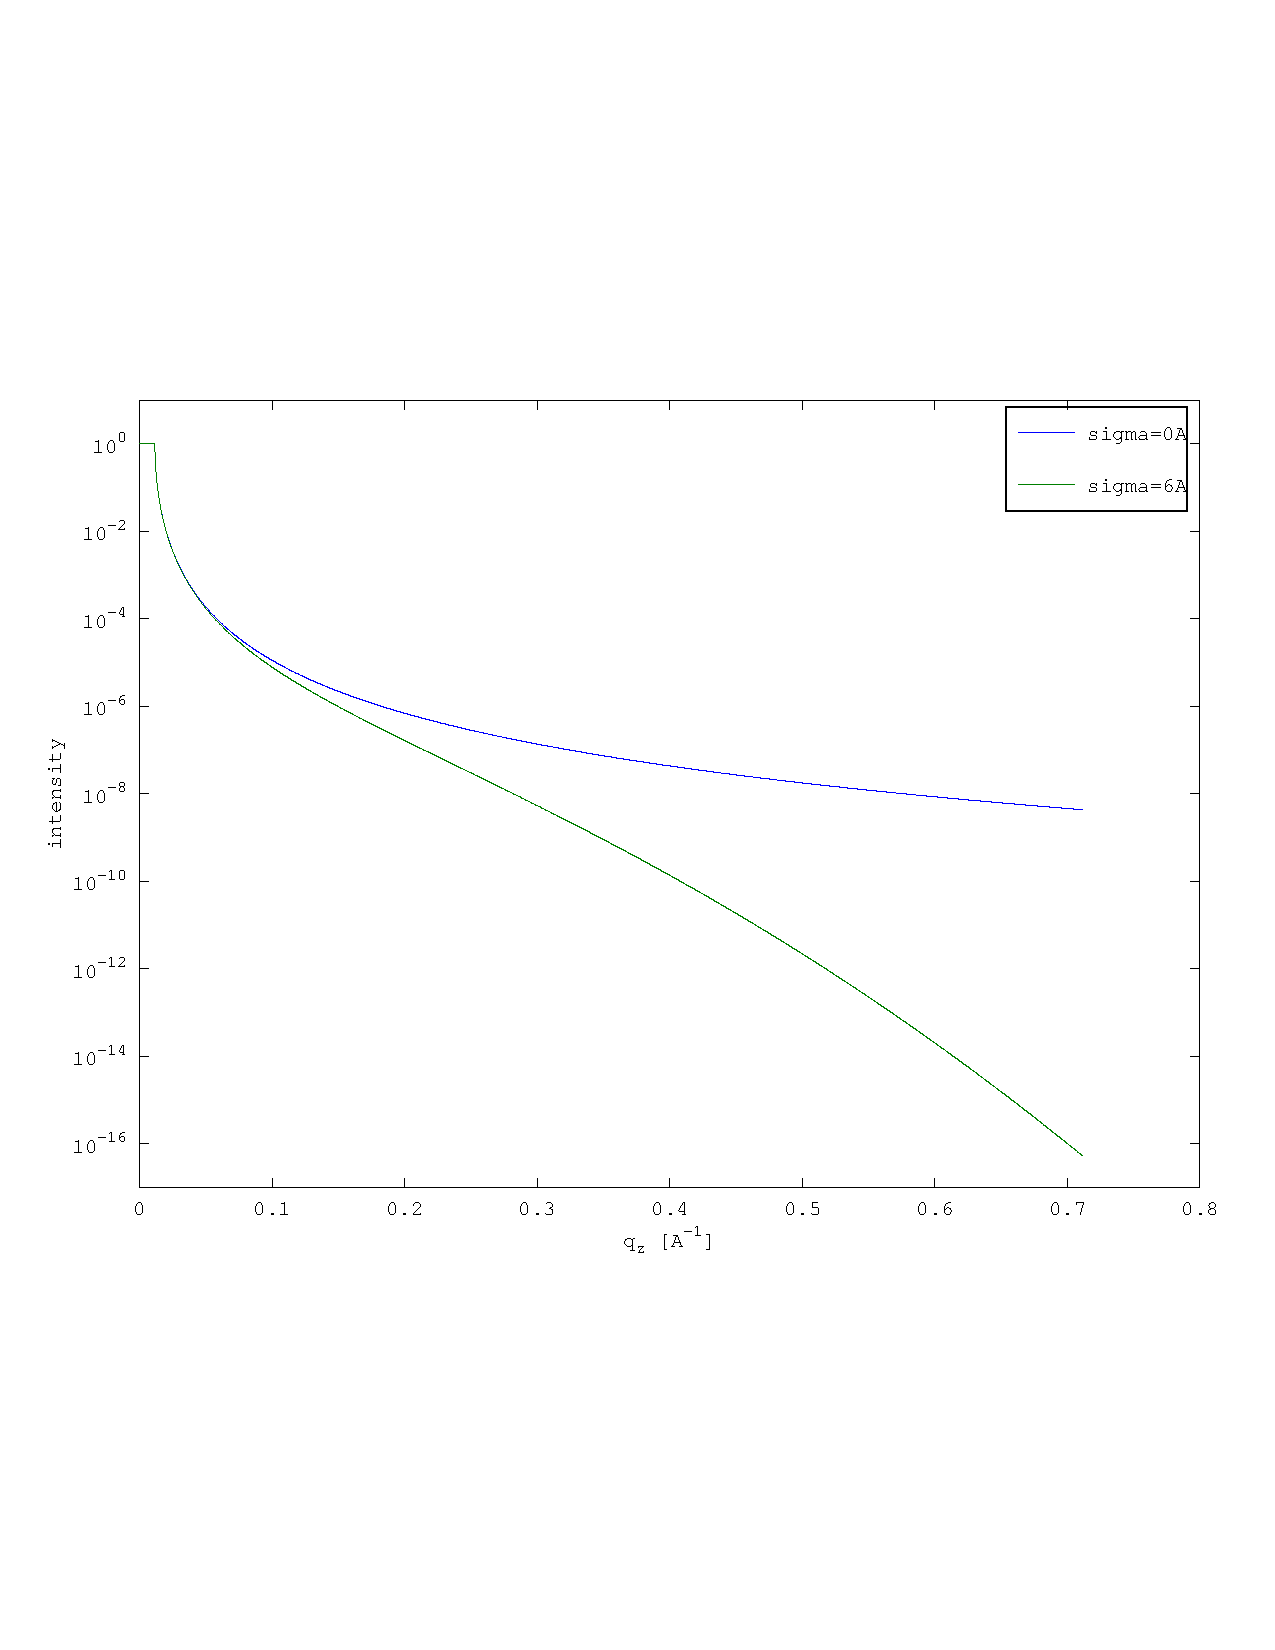
\includegraphics[width=10cm]{images/reflektivitaet_rau.pdf}
	\captionof{figure}{Berechnete Reflexität für ein Substrat mit unterschiedlichen Rauigkeiten $\sigma_1=$\SI{0}{\angstrom} und $\sigma_2=$\SI{6}{\angstrom}.}
	\label{fig:rauigkeitbeispiel}
\end{center}
\subsection{Geometrischer Winkel}
Bei kleinen Winkeln trifft der Röntgenstrahl nicht vollständig auf die Probe. Der Winkel, ab dem der gesamte Strahl auf die Probe trifft wird als Geometriewinkel 
\begin{align}
\alpha_{\indx{g}}=\arcsin \left( \frac{d_0}{D} \right)
\end{align}
bezeichen. 
Dabei ist $D$ der Durchmesser der Probenoberfläche und $d_0$ die Höhe des Strahls.
Es lässt sich so ein Geometriefaktor 
\begin{align}
G=\left\lbrace\begin{matrix}
\frac{D \sin \alpha_{i} }{d} &,\ \alpha_{i} < \alpha_{\indx{g}} \\
1 &,\  \alpha_{i} > \alpha_{\indx{g}}
\end{matrix}\right.
\end{align}
bestimmen, der angibt, welcher Anteil des Strahls auf die Probenoberfläche trifft.
Der Geometriefaktor muss reziprok mit der gemessenen Itensität multiplizert werden.
\section{Aufbau}
$I\left(\vec{k}\right)=\left\|\Psi_0\left(\vec{k}\right)+\sum\limits_j\Psi_j\left( \vec{k} \right) \right|^2$

\section{Durchführung}

\subsection{Justage des D8-Labordiffraktometers}

\subsection{Messung der Röntgenreflektivität}

\section{Auswertung}

\subsection{Diffuser Scan}
In Abbildung \ref{fig:diffus} sind der diffuse Scan, die Originalmessdaten und die bereinigten Daten dargestellt. Die weitere Datenverarbeitung wird mit den bereinigten Daten durchgeführt.

\begin{center}
	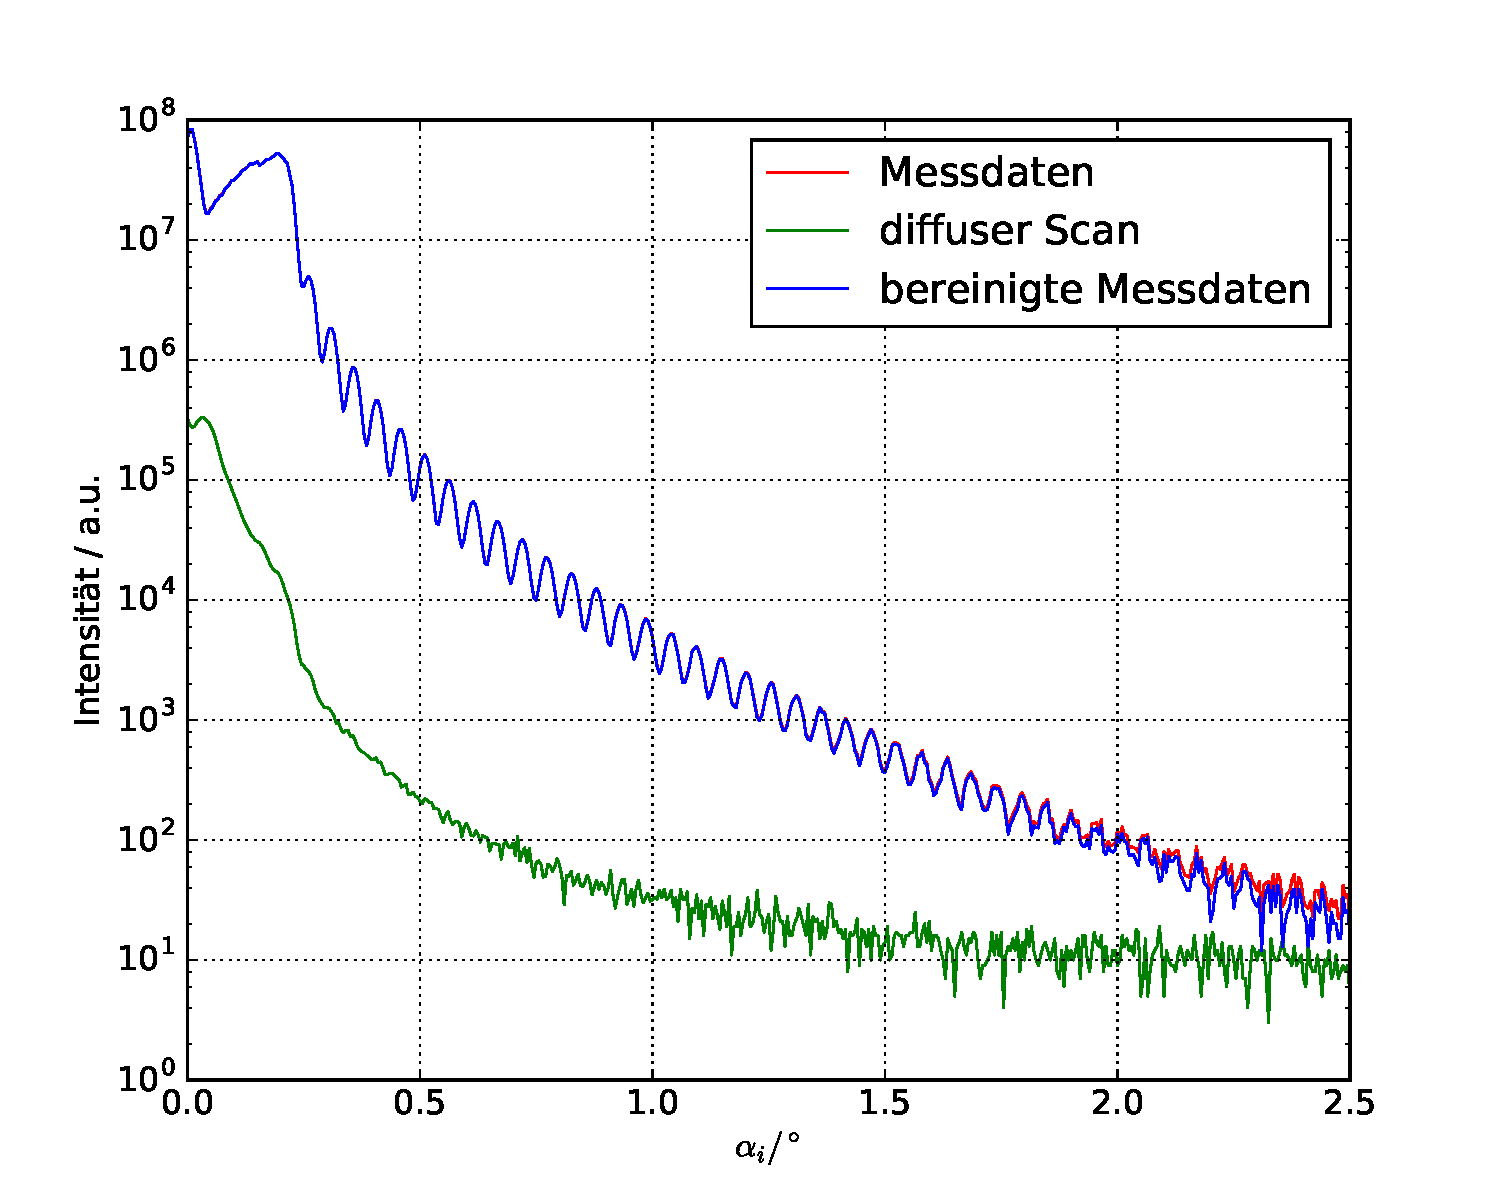
\includegraphics[width=0.8\textwidth]{images/rawdata.pdf}
	\captionof{figure}{Messwerte der Primär- und der Diffusmessung}
	\label{fig:diffus}
\end{center}

\subsection{Geometriewinkel und Geometriefaktor}
Der Geometriewinkel konnte aus dem Rockingscan zu
\begin{align*}
\alpha_G=0.3247^{\circ}
\end{align*}
bestimmt werden. \\
Zur Berechnung der Schichtdicke
\section{Brechungsindex und Rauigkeit}

\section{Diskussion}

\section{Quellen}
%\renewcommand{\labelenumi}{\value{enumi}}
\begin{enumerate}[label={[\arabic*]}]
\item \label{q:anleitung} \textbf{Physikalisches Praktikum}, TU Dortmund: \\
\textit{Versuchsanleitung zu Versuch: Röntgenreflektometrie} \\
\url{http://e1.physik.tu-dortmund.de/cms/Medienpool/Downloads/Roentgenreflektometrie_Versuch.pdf} (letzte Version vom 15.02.2017, 12:26)
\end{enumerate}

\end{document}